\chapter{\ifenglish Background Knowledge and Theory\else ทฤษฎีที่เกี่ยวข้อง\fi}
การทําโครงงาน เริ่มต้นด้วยการศึกษาค้นคว้า ทฤษฎีที่เกี่ยวข้อง หรือ งานวิจัย/โครงงาน ที่เคยมีผู้นําเสนอ
ไว้แล้ว ซึ่งเนื้อหาในบทนี้ก็จะเกี่ยวกับการอธิบายถึงสิ่งที่เกี่ยวข้องกับโครงงาน เพื่อให้ผู้อ่านเข้าใจเนื้อหาในบท
ถัดๆ ไปได้ง่ายขึ้น
\section{Mobile operating systems}
\subsection{ระบบปฎิบัติการแอนดรอยด์(Android OS)}

\subsubsection{ประวัติและความเป็นมาของระบบปฏิบัติการแอนดรอยด์}

เริ่มต้นระบบปฏิบัติการแอนดรอยด [5] ถูกพัฒนามาจากบริษัท แอนดรอยด์(Android Inc.) เมื่อปี
พ.ศ 2546 โดยมีนาย แอนดี้ รูบิน (Andy Rubin) ผู้ให้กําเนิดระบบปฏิบัติการนี้ และถูกบริษัท กูเกิ้ล ซื้อ
กิจการเมื่อ เดือนสิงหาคม ปี พ.ศ 2548 โดยบริษัทแอนดรอยด์ ได้กลายเป็นมาบริษัทลูก ของบริษัทกูเกิ้ล
และยังมีนาย แอนดี้ รูบิน ดําเนินงานอยู่ในทีมพัฒนาระบบปฏิบัติการต่อไป

ระบบปฏิบัติการแอนดรอยด์ เป็นระบบปฏิบัติการที่พัฒนามาจากการนําเอา แกนกลางของระบบปฏิบัติ
การลินุกซ์(Linux Kernel) ซึ่งเป็นระบบปฏิบัติการที่ออกแบบมาเพื่อทํางานเป็นเครื่องให้บริการ (Server)
มาพัฒนาต่อ เพื่อให้กลายเป็นระบบปฏิบัติการบนอุปกรณ์พกพา (Mobile Operating System)

ต่อมาเมื่อเดือน พฤศจิกายน ปี พ.ศ 2550 บริษัทกูเกิ้ล ได้ทําการก่อตั้งสมาคม OHA (Open Handset Alliance, http://www.openhandsetalliance.com) เพื่อเป็นหน่วยงานกลางในการกําหนดมาตรฐานกลาง ของอุปกรณ์พกพาและระบบปฏิบัติการแอนดรอยด์ โดยมีสมาชิกในช่วงก่อนตั้งจํานวน 34 ราย
เข้าร่วม ซึ่งประกอบไปด้วยบริษัทชั้นนําที่ดําเนินธุรกิจด้าการสื่อสาร เช่น โรงงานผลิตอุปกรณ์พกพา, บริษัท
พัฒนาโปรแกรม, ผู้ให้บริการสื่อสาร และผู้ผลิตอะไหล่อุปกรณ์ด้านสื่อสาร


\subsubsection{ประเภทของระบบปฎิบัติการ Android}
เนื่องจากระบบปฎิการ android เป็น ซอฟต์แวร์เปิ ด จึงอนุญาติให้นักพัฒนาหรือผู้ที่สนใจ สามารถดาวน์-
โหลด Sorce Code ได้ ทําให้มีผู้พัฒนาจากหลายๆ ฝ่ ายนํา Source Code มาปรับแต่วและพัฒนาสร้างแอพ
พลิเคชั่นบนระบบ Android ในแบบฉบับของตนเองมากขึ้น โดยมาสามารถแย่งประเภทของระบบ android
ออกเป็นกลุ่มๆ ได้3 ประเทําดังต่อไปนี้

Android Open Sorce Project (AOSP) เป็นระบบ Android ประเภทแรกที่ทางบริษัท google
เปิดให้สามารถนํา Source Code ไปติดตั้งและใช้งานในอุปกรณ์ ได้โดยไม่ต้องไปเสียค่าใช่จ่าย

Open Handset Mobile (OHM) เป็นแอนดรอย์ที่ได้รับการพัฒนากับกลุ่ม Open Handset ALLiances (OHM) ซึ่งบริษัทเหล่านี้จะพัฒนาระบบ Android ในแบบฉบับของตนเอง โดยมีรูปร่าง หน้าตา
การแสดงผล และฟั งกืชัน การใช้งานที่แตกต่างกัน รวมไปถึงอาจจะมีความเป็นเอกลักษณ์ และรูปแบบการ
ใช้งานเป็นของงแต่ละบริษัท และ program Android ประเภทนี้ก็จะได้รับสิทธิ์ บริการเสริมต่างๆ จาก
Google ที่เรียกว่า GMS (Google Mobile Service) ซึ่งเป็นบิการเสริมที่ ทําให้ระบบ Android มี
ประสิทธิภาพขึ้นนั้นเอง

Cooking หรือ Customize เป็น ระบบ Android ที่นักพัฒนานําเอาซอร์สโค้ตจากแหล่งต่างๆ มาประ
บแต่งให้อยุ่ในแบบฉบัยของตนเอง ซึ่งการพัฒนาจะต้องปลดล็อกสิทธิ์ในการใช้งานอุปกรณ์(Unlock) เสีย
ก่อนจึงจะสามารถติดตั้งได้ ทั้งนี้ระบบ Android ประเภทนี้ ถือได้ว่าเป็นประเภทที่มีความสามารถสูงที่สุด
เนื่องจากจะได้รับการปรับแต่งขีดความสามารถต่างๆ ให้มีเข้ากันได้กับอุปกรณ์นั้นๆ จากผู้ใช้งานจริง


\subsubsection{สถาปัตยกรรมของระบบแอนดรอยด์}
\begin{figure}[h]
  \begin{center}
    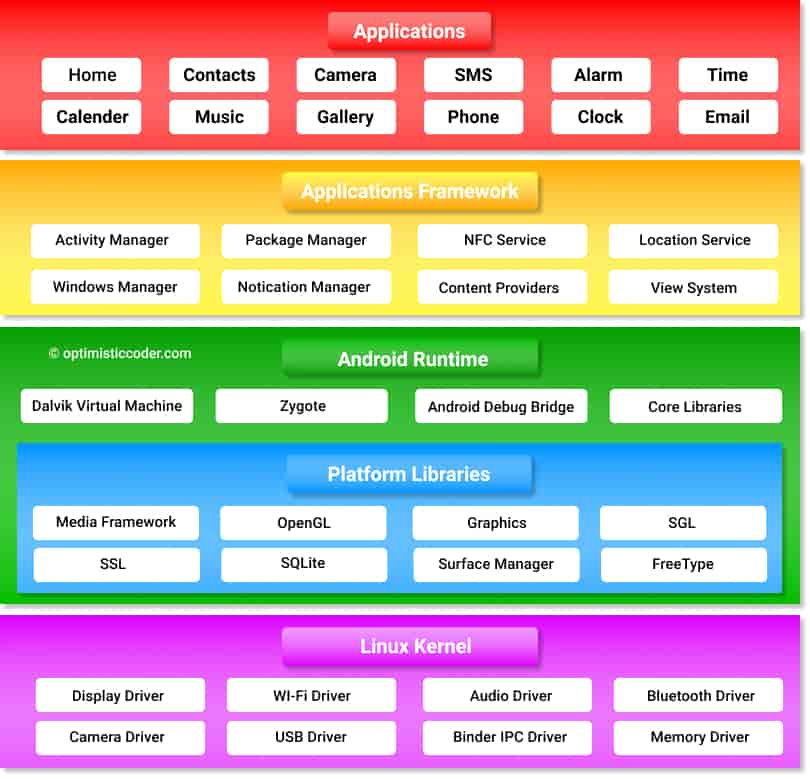
\includegraphics[width=0.8\textwidth]{./image/architecture.jpg}
  \end{center}
  \caption[Poem]{android architecture}
  \label{fig:walrus}
  \end{figure}

\begin{enumerate}
    \item ชั้นแอพพลิเคชัน(Application) ชั้นนี้เป็นชั้นบนสุดของโครงสร้าง Android ซึ่งเป็นส่วน ของแอพพลิเคชันที่พัฒนาขึ้นมาใช้งาน เช่น แอพพลิเคชันรับส่งอีเมลล์ แอพพลิเคชันโทรศัพท์(Phone Dial) แอพพลิ-
    เคชันเว็บบราวเซอร์(Web Browser) เป็นต้น ทั้งนี้โปรแกรมในชั้น แอพพลิเคชันนั้นจะอยู่ ในรูปแบบของ
    ไฟล์.apk ซึ่งโดยทั่วไปแล้วจะอยู่ในไดเร็คทอรี่ data/app ของ โทรศัพท์
    
    \item ชั้นแอพพลิเคชันเฟรมเวิร์ค (Application Framework) โดยปกติแล้วนักพัฒนาสามารถ เรียกใช้
    งาน Android ผ่าน API (Application Programming Interface) ได้ ซึ่ง Android ได้ออกแบบ ไว้
    เพื่อลดความซ้า ซ้อนในการใช้งานซ้า ของ Application Component
    \item ชั้นไลบรารี(Library) แอนดรอยด์ได้รวบรวมกลุ่มของไลบรารีต่างๆ ที่สาคัญและมีความ จา เป็นต่อ
    การพัฒนาโปรแกรมเอาไว้มากมา ซึ่งถูกเขียนไว้ด้วยภาษา C และ C++

    \item ชั้นลีนุกซ์เคอร์เนล (Linux Kernel) ระบบ Android อยู่บนพื้นฐานของระบบปฏิบัติการ Linux
    โดยชั้น Linux Kernel นั้นมีฟั งก์ชันการทา งานหลายๆส่วน ซึ่งแต่ละส่วนถูกพัฒนาขึ้นด้วย ภาษา C เช่น
    การจัดการหน่วยความจา (Memory Management) การจัดการโพรเซส (Process Management) การ
    เชื่อมต่อเครือข่าย(Networking) และฟั งก์ชันการทางานส่วนอื่นที่เกี่ยวข้องกับ ระบบ ปฏิบัติการ ทั้งนี้นัก
    พัฒนาจะไม่มีสิทธ์ิ
    เข้าถึงส่วนนี้ได้โดยตรง ซึ่งนักพัฒนาสามารถเข้าถึง ระบบปฏิบัติ การ Linux ได้จากชุดคา
    สั่ง Command Prompt เช่น adb shell ซึ่งจะสามารถใช้ เครื่องมือต่างๆ ได้ เช่น การเข้าดูระบบไฟล์(File
    System) โพรเซสการคัดลอกไฟล์(Copy File) เป็นต้น
    
\end{enumerate}
\section{Development tools and technology}
\subsection{Firebase}
Firebase [9] คือ Platform ที่รวบรวมเครื่องมือต่าง ๆ สําหรับการจัดการในส่วนของ Backend หรือ
Server side ซึ่งทําให้สามารถ Build Mobile Application ได้อย่างมีประสิทธิภาพ และยังลดเวลาและ
ค่าใช้จ่ายของการทํา Server side หรือการวิเคราะห์ข้อมูลให้อีกด้วย โดยมีทั้งเครื่องมือที่ฟรี และเครื่องมีที่
มีค่าใช้จ่าย (สําหรับการ Scale)

\subsubsection{ผลิตภัณฑ์ต่าง ๆ ของ Firebase}
Firebase มีผลิตภัณฑ์ทั้งหมดถึง 18 อย่างและแบ่งออกเป็น 3 หมวดหมู่ ดังนี้

\subsubsection{Build better apps}
มีทั้งหมด 7 ผลิตภัณฑ์ ได้แก่
\begin{enumerate}
  \item Realtime Database คือบริการฐานข้อมูล NoSQL ใช้วิธีการเก็บข้อมูลเป็น JSON Tree
  ขนาดใหญ่ และสามารถ Sync สถานะข้าม Client ได้แบบ Realtime กล่าวคือ หากเชื่อมต่อ Database
  เดียวกัน 2 ที่ เมื่อใดที่ที่นึงมีการอัพเดตข้อมูล อีกที่นึงก็จะมีการอัพเดตข้อมูลให้เหมือนกันโดยอัตโนมัติ และ
  สามารถทํางานแบบ Offline ได้บนแอป Android และ iOS
  
  \item Authentication คือบริการตรวจสอบผู้ใช้ โดยสามารถตรวจสอบได้หลายวิธี เช่น Email/Password, เบอร์โทรศัพท์, บัญชีGoogle, Facebook, Twitter, Github เป็นต้น มีฐานข้อมูลเป็นของตัวเอง
  ไม่ต้องสร้างใหม่หรือออกแบบวิธีการเก็บซึ่ง สามารถดูได้ว่าสมัครด้วยวิธีไหน สมัครเมื่อไหร่ และเข้าใช้ระบบ
  ครั้งล่าสุดเมื่อไหร่
  
  \item  Hosting คือบริการฝากไฟล์static เช่น HTML, CSS, JS, JPG(ไม่รองรับ PHP ซึ่งเป็น
  Dynamic) เพื่อให้คนอื่น ๆ เข้าใช้งานเว็บของเราได้ มักนิยมใช้ในการฝากไฟล์ที่ได้จากการ Build ของ
  JavaScript Framework ต่าง ๆ เช่น Angular, React, Vue สังเกตว่าจะได้ไฟล์HTML, CSS, JS
  ต่าง ๆ ตามที่ได้บอกไว้ข้างต้น หรือจะเป็นไฟล์ที่เขียนเองก็ได้ ไม่จําเป็นต้องใช้Framework ก็ได้เหมือนกัน
  อีกทั้งมีCDN และ SSL มาด้วยแบบฟรี ๆ เพื่อให้ผู้ใช้ของคุณได้รับประสบการณ์การใช้งานที่ปลอดภัยเชื่อถือได้และไม่มีความล่าช้าแม้ว่าจะอยู่ที่ไหนก็ตาม ทุกเว็บมีDomain Name ของ Firebase ให้อัตโนมัติ แต่
  เปลี่ยนมาใช้ของตัวเองได้

  \item Cloud Functions คือบริการสําหรับ Deploy Function ที่พัฒนาด้วย JavaScript หรือ
TypeScript เพื่อทํางานตาม Tigger (คล้าย ๆ event) ที่เกิดขึ้นบน Firebase เช่น ถ้า Database ถูก
เขียน (Realtime Database Triggers) ให้Function เราส่ง Notification แจ้งไปบอกเราด้วย หรือ มี
การเรียนมาที่ HTTP Endpoint (HTTP Triggers) ให้Function เราคืนค่า HTML กลับไป (ใช้ทํา
REST API) หรือ ถ้าแอปมีปัญหา (Crashlytics Triggers) ให้ส่งข้อความแจ้งเตือนไปที่ Slack

  \item Cloud Storage คือบริการเก็บไฟล์รูปภาพ, ไฟล์เสียง, วิดีโอ เพื่อใช้บน Application เช่น
  รูปภาพประจําตัวสมาชิก, วิดิโอสอนการใช้งานโปรแกรม เป็นต้น
  \item Cloud Firestore (Beta) คือ Realtime Database รุ่นใหม่มาพร้อมการค้นหาและการปรับ
  ขนาดอัตโนมัติที่มีประสิทธิภาพมากขึ้น ปรับปรุงวิธีการเก็บข้อมูลใหม่เป็น Collections และสามารถทํางาน
  แบบ Offline บน Web ได้อีกด้วย (จากเดิมทําได้แค่บน Android และ iOS)
  \item ML Kit (Beta) คือ Machine Learning SDK ที่ช่วยให้แอปมือถือสามารถใช้ความสามารถ
  ของ ML ได้ง่ายยิ่งขึ้น สามารถทํางานได้ทั้งแบบ Online และ Offline
\end{enumerate}

\subsubsection{Improve app quality}
มีทั้งหมด 3 ผลิตภัณฑ์ ได้แก่
\begin{enumerate}
  \item Crashlytics คือบริการตรวจจับและแจ้งเตือนหากแอปเราเกิดอาการ Crash ขึ้นแบบ Realtime
  เพื่อให้แอปเราเสถียรอยู่เสมอ โดยจะทําการแจ้งให้ทราบถึงข้อผิดพลาดและผลกระทบ ผ่านทาง E-mail และ
  Firebase Console (ใช้Cloud Functions เพื่อส่งไปที่อื่นด้วยได้ เช่น slack) เพื่อการแก้ปัญหาที่รวดเร็ว
  และตรงจุด
  
  \item Performance Monitoring คือบริการตรวจสอบคุณภาพของแอป เพื่อให้แอปของเราตอบสนอง
  ได้เร็วอยู่เสมอ โดยสามารถตรวจสอบเวลาและรายละเอียดการทํางานต่าง ๆ เช่น เวลาที่ใช้ในการเปิ ดแอป ,
  เวลาที่ใช้การเปลี่ยนหน้า UI, เวลาที่ใช้ในการโหลด API, ขนาดข้อมูลที่ Download/Upload, จํานวน
  API ที่สําเร็จหรือล้มเหลว เป็นต้น
  
  \item  Test Lab คือบริการทดสอบแอปบนฮาร์ดแวร์จริง ๆ เพื่อให้มั่นใจว่าแอปของเราสามารถรองรับ
  ฮาร์ดแวร์ที่เราต้องการได้จริง ๆ โดยสามารถระบุรุ่นและเวอร์ชันที่ต้องการได้ แล้วระบุรูปแบบการทดสอบต่าง
  ๆ เพื่อทดสอบและรายงานผลกลับมา ไม่ต้องซื้อโทรศัพท์เอง (สมมุติว่าจริงจังเรื่องการรองรับทุกอุปกรณ์มาก)
  ซึ่งเป็นเรื่องยากด้วยหากจะซื้อทุกรุ่นที่คนนิยมใช้ในตลาด ไหนจะต่อสาย จะนั่งทดสอบทีละเครื่องอีก ใช้ตัวนี้
  จบ หมดปัญหา
\end{enumerate}

\subsubsection{Grow your business}
มีทั้งหมด 8 ผลิตภัณฑ์ ได้แก่ 
\begin{enumerate}
  \item  In-App Messaging คือบริการแสดงข้อความ pop-up ภายในแอป
  ของเรา เช่น โฆษณา (เจอประจําเลย), การแจ้งเตือน, ข่าวสาร เป็นต้น

  \item  Google Analytics คือบริการแสดงข้อมูลสถิติต่าง ๆ ของแอป เช่น ใช้ด้วยระบบปฏิบัติการอะไร
  จํานวนเท่าไหร่, มีผู้ใช้งาน ณ ปั จจุบันกี่คน, ใช้งานส่วนไหนบ้าง เป็นต้น เพื่อวิเคราะห์กลุ่มเป้ าหมาย หรือรับ
  ทราบพฤติกรรมของผู้ใช้งานต่าง ๆ
  
  \item Predictions คือบริการวิเคราะห์ข้อมูลการใช้งานแอป ช่วยให้เรารู้ว่าผู้ใช้ใช้งานส่วนใดบ้างในแอป
  ช่วยให้เรารู้ว่าส่วนใดตอบสนองได้ดี ส่วนใดควรปรับปรุง หรืออาจต้องการที่จะหยั่งรู้พฤติกรรมในอนาคตของ
  ผู้ใช้งานแอปของคุณ เพื่อวางแผนกลยุทธ์ทั้งรุกและรับ รวมทั้งสร้างประสบการณ์ที่น่าประทับใจให้กับผู้ใช้ของ
  เรา
  \item Cloud Messaging คือบริการส่งการแจ้งเตือนไปยังมือถือหรือเว็บของเรา เพื่อแจ้งข้อความไป
  ยังผู้ใช้ของเราแม้ว่าจะปิ ดแอปไปแล้วก็ตาม ถ้าใครใช้Smartphone อยู่(น่าจะทุกคนแหละ ที่กําลังอ่านบทความนี้อยู่) จะคุ้นเคยกันเป็นอย่างดี เช่น การแจ้งเตือนจาก facebook, line, instagram ต่าง ๆ เป็นต้น
  
  \item    Remote Config คือความสามารถที่จะเปลี่ยนลักษณะการทํางานและลักษณะที่ปรากฏของแอป
  ของคุณได้ทันทีจากหน้าเว็บ Firebase โดยไม่ต้องรอการอนุมัติจาก App Store เช่น การเปลี่ยนรูปแบบ
  ตามเทศกาล, เปลี่ยนภาษาตามผู้ใช้งาน เป็นต้น
  \item   Dynamic Links คือลิ้งค์เชื่อมโยงไปยังแอปมือถือ ใช้สําหรับแสดงบนหน้าเว็บเพื่อให้ผู้ใช้งานติด
  ตั้งแอปมือถือผ่านลิ้งค์ลิ้งค์นี้ อีกทั้งยังสามารถแนบข้อมูลต่าง ๆ ของผู้ใช้ที่อยู่บนเว็บมาด้วยได้  
  \item    App Indexing คือการปรับแต่งแอปของเราให้แสดงผลข้อมูลภายในแอปบน Google Search
  ได้(เรียกการทํา SEO แบบ Mobile App ก็คงไม่ผิด) เช่น ค้นชื่อร้านอาหารแล้วปรากฏแอปวงในขึ้นมาให้
  ดูรายละเอียดและรีวิว เป็นต้น
  
  \item   A/B Testing (Beta) คือความสามารถในการแสดงผลแอปหลายรูปแบบเพื่อทดสอบการแสดง
  ผลหรือการทํางาน ว่าสิ่งไหนจะมอบประสบการณ์การใช้งานที่ดีกว่าให้แก่ผู้ใช้งาน เช่น การวางป่ ุมกดแบบ
  ไหนที่ผู้ใช้งานใช้สะดวก สมมุติว่ามีผู้ใช้งาน 100 คน อาจจะมี50 คนได้ป่ ุมที่อยู่มุมบน อีก 50 คนได้ป่ ุมอยู่
  มุมล่าง หากว่ามีการใช้งานแบบไหนมากกว่ากันก็อาจจะสรุปผลและเลือกใช้แบบนั้นกับทุกคนในท้ายที่สุด

\end{enumerate}

\subsection{Android Studio}
Android Studio [6] เป็น IDE Tool จาก Google ไว้พัฒนา Android สําหรับ Android Studio
เป็น IDE Tools ล่าสุดจาก Google ไว้พัฒนาโปรแกรม Android โดยเฉพาะ โดยพัฒนาจากแนวคิดพื้น
ฐานมาจาก InteliJ IDEA คล้าย ๆ กับการทํางานของ Eclipse และ Android ADT Plugin โดยวัตถุ-
ประสงค์ของ Android Studio คือต้องการพัฒนาเครื่องมือ IDE ที่สามารถพัฒนา App บน Android ให้
มีประสิทธิภาพมากขึ้น ทั้งด้านการออกแบบ GUI ที่ช่วยให้สามารถ Preview ตัว App มุมมองที่แตกต่างกัน
บน Smart Phone แต่ล่ะรุ่น สามารถแสดงผลบางอย่างได้ทันทีโดนไม่ต้องทําการรัน App บน Emulator
รวมทั้งยังแก้ไขปรับปรุงในเรื่องของความเร็วของ Emulator ที่ยังเจอปัญหากันอยู่ในปั จจุบัน

\subsection{JSON (Java Script Object Notation)}
JSON [8] ย่อมาจากคําว่า Java Script Object Notation เป็นฟอร์แมตสาหรับการแลกเปลี่ยนข้อมูล
ที่มีขนาดเล็ก ซึ่งสามารถทําความเข้าใจได้ง่าย และสามารถถูกสร้างและอ่านโดยเครื่องได้ง่าย ซึ่ง JSON ถูก
กําหนดให้อยู่ภายใต้ภาษา Java Script (Java Script Programming Language,Standard ECMA262
3rd Edition - December 1999.) ที่มีรูปแบบข้อมูลตัวอักษรที่มีความอิสระอย่างสมบูรณ์ แต่จะ มีหลัก
การเขียนคุ้นเคยกับนักเขียนโปรแกรมภาษาต่างๆ เช่น ภาษา C, C++, Java, Javascript, Perl, Phython
และอื่นๆ คุณสมบัติเหล่านี้ทําให้JSON เป็นภาษาในการแลกเปลี่ยนข้อมูลที่มีความ สมบูรณ์แบบ ประเภท
ของ JSON
\begin{enumerate}
  \item  Client-server architecture: Client ไม่จําเป็นต้องรู้อะไรเกี่ยวกับ Business logic ภายใน ไม่มี
  หน้าที่เกี่ยวกับการจัดเก็บข้อมูล ส่วน Server มีหน้าที่เก็บ Resource และไม่จําเป็นต้องรู้อะไรเกี่ยว
  กับ UI Frontend หรือสถานะของผู้เรียก
  

  \item  Number: ตัวเลขเท่านั้น
  
  \item String: Unicode ใช้เครื่องหมาย double-quote (“) เป็นตัวบ่งบอก และสามารถใช้backslash
  syntax ได้
  
  \item Boolean: True or False
  \item    Array: ชุดข้อมูล ซึ่งจะเป็นชนิดใดก็ได้ ใช้สัญลักษณ์square bracket [var1,var2] เป็นตัวแสดง
  และคั้นด้วย comma แต่ะลค่าใน array
  \item  Object: ชุดข้อมูลที่เป็นคู่Key-Value แบบ strings [key1:value1, key2:value2] ใช้comma
  เป็นตัวแบ่งแต่ละคู่ และใช้colon เป็นตัวแบ่งระหว่าง key และ value
  \item    Null: ค่าว่าง
\end{enumerate}

\subsection{NoSQL Databases}
ฐานข้อมูล NoSQL [1] สร้างตามวัตถุประสงค์สําหรับโมเดลข้อมูลแบบเฉพาะเจาะจงและมีแบบแผนที่
ยืดหยุ่นสําหรับการสร้างแอปพลิเคชันอันทันสมัย ฐานข้อมูล NoSQL เป็นที่รู้จักกันดีในด้านความง่ายในการ
พัฒนา การทํางาน และประสิทธิภาพตามขนาดที่ต้องการ หน้านี้ประกอบด้วยทรัพยากรเพื่อช่วยให้คุณเข้าใจ
ฐานข้อมูล NoSQL และเริ่มต้นใช้งาน
\subsection{Android SDK}
Android Software Development Kit (Android SDK) [7] เปรียบเสมือน Library ที่ใช้ใน
การพัฒนา Application สําหรับ Android เนื่องจากตัว Android มีหลายเวอร์ชั่นและแต่ละเวอร์ชั่นมี
Feature, GUI ที่ไม่เหมือนกันทําให้เกิด Android SDK ออกมาหลายเวอร์ชั่นให้เลือกใช้งาน

\subsection{JDK (Java Development Kit)}
Java Development Kit หรือ JDK [2] คือชุดของเครื่องมือที่ใช้ในการพัฒนาโปรแกรม JAVA ของ
บริษัทซัน ไมโครซิสเต็มส์ นักกพัฒนาโปรแกรมโดยใช้ภาษา Java อย่างเช่น Java Compiler, Java Debugger, Java Doc และ Java Interpreter หรือ Java VM จะต้องติดตั้ง JDK นี้ ไม่ งั้นจะไม่สามารถ
Compile และ Run java ได้ เวอร์ชันปั จจุบันของ JDK คือเวอร์ชั่น 7 ประกอบไป ด้วยโปรแกรมต่างๆ
อาทิเช่น โปรแกรม คอมไพเลอร์(javac.exe) โปรแกรมอินเตอร์พรีตเตอร์(java.exe) โปรแกรมดีบักเกอร์
แต่จะไม่มีโปรแกรม อีดิเตอร์
\begin{enumerate}
  \item  Java SE (Standard Edition) สําหรับพัฒนาโปรแกรมบนคอมพิวเตอร์ตั้งโต๊ะทั่วไป
  
  \item  Java ME (Micro Edition) สําหรับพัฒนาโปรแกรมบนอุปกรณ์พกพา เช่น โทรศัพท์มือถือหรือพี
  ดีเอ ส่วนมากใช้เขียนโปรแกรมเกม
  
  \item Java EE (Enterprise Edition) สําหรับพัฒนาโปรแกรมในองค์กรใหญ่ๆ หรือมี ขอบเขตของโครงการกว้างมาก
\end{enumerate}
\subsection{SDK Platform (Software Development Kit )}
SDK [3] ซึ่งย่อมาจาก Software Development Kit คือเครื่องมือที่เอาไว้สําหรับพัฒนาโปรแกรมหรือ
แอพพิเคชั่นบนระบบ Android OS ซึ่งทาง Google พัฒนาออกมาเพื่อแจกจ่ายให้นักพัฒนาแอพพลิเคชั่น
หรือผู้สนใจทั่วไปดาวน์โหลดไปใช้กันโดยไม่มีค่าใช้จ่าย และนี่ก็เป็นหนึ่งในปั จจัยที่ทําให้แอพพลิเคชั่นบนแอน
ดรอยด์นั้นเพิ่มขึ้น อย่างรวดเร็ว ซึ่งในชุด SDK นั้นจะมีโปรแกรมและไลบรารี่ต่างๆ ที่จําเป็นต่อการพัฒนา
แอพพลิเคชั่นบนแอนดรอยด์ อย่างเช่น Emulator ซึ่งทําให้ผู้ใช้สามารถสร้างแอพพลิเคชั่นและนํามาทดลอง
รันบนตัวอีมูเลเตอร์ ก่อน โดยมีสภาวะแวดล้อมเหมือนมือถือที่รันระบบปฏิบัติการแอนดรอยด์จริงๆ
\subsection{AVD (Android Visual Device)}
การทําแอพพลิเคชั่นสําหรับแอนดรอยจะมีส่วนที่ต้องทดสอบแอพที่ทําขึ้นมากับอุปกรณ์โทรศัพท์หรือแท็บเล็ต เพื่อดูผลลัพธ์ของแอพ ในตัว Android Studio มีเครื่องมือ Android Virtual Device (AVD) [4]
เพื่อให้ในการทดสอบแอพโดยเราสามารถสร้างตัวจําลองโทรศัพท์และแท็บเล็ตขึ้นมาเองได้ โดยสามารถเลือก
ขนาดหน้าจอ และเวอร์ชั่นของตัวแอนดรอยให้ตรงตามความต้องการได้


% \begin{equation}\label{eq:dielectric}
% k_1=\frac{\omega}{c({1/\varepsilon_m + 1/\varepsilon_i})^{1/2}}=k_2=\frac{\omega
% \sin(\theta)\varepsilon_\mathit{air}^{1/2}}{c}
% \end{equation}

% \noindent
% where $\omega$ is the frequency of the plasmon, $c$ is the speed of
% light, $\varepsilon_m$ is the dielectric constant of the metal,
% $\varepsilon_i$ is the dielectric constant of neighboring insulator,
% and $\varepsilon_\mathit{air}$ is the dielectric constant of air.

% \section{About using figures in your report}

% % define a command that produces some filler text, the lorem ipsum.
% \newcommand{\loremipsum}{
%   \textit{Lorem ipsum dolor sit amet, consectetur adipisicing elit, sed do
%   eiusmod tempor incididunt ut labore et dolore magna aliqua. Ut enim ad
%   minim veniam, quis nostrud exercitation ullamco laboris nisi ut
%   aliquip ex ea commodo consequat. Duis aute irure dolor in
%   reprehenderit in voluptate velit esse cillum dolore eu fugiat nulla
%   pariatur. Excepteur sint occaecat cupidatat non proident, sunt in
%   culpa qui officia deserunt mollit anim id est laborum.}\par}

% \begin{figure}
%   \centering

%   \fbox{
%      \parbox{.6\textwidth}{\loremipsum}
%   }

%   % To include an image in the figure, say myimage.pdf, you could use
%   % the following code. Look up the documentation for the package
%   % graphicx for more information.
%   % \includegraphics[width=\textwidth]{myimage}

%   \caption[Sample figure]{This figure is a sample containing \gls{lorem ipsum},
%   showing you how you can include figures and glossary in your report.
%   You can specify a shorter caption that will appear in the List of Figures.}
%   \label{fig:sample-figure}
% \end{figure}

% Using \verb.\label. and \verb.\ref. commands allows us to refer to
% figures easily. If we can refer to Figures
% \ref{fig:walrus} and \ref{fig:sample-figure} by name in the {\LaTeX}
% source code, then we will not need to update the code that refers to it
% even if the placement or ordering of the figures changes.

% \loremipsum\loremipsum

% % This code demonstrates how to get a landscape table or figure. It
% % uses the package lscape to turn everything but the page number into
% % landscape orientation. Everything should be included within an
% % \afterpage{ .... } to avoid causing a page break too early.
% \afterpage{
%   \begin{landscape}
%   \begin{table}
%     \caption{Sample landscape table}
%     \label{tab:sample-table}

%     \centering

%     \begin{tabular}{c||c|c}
%         Year & A & B \\
%         \hline\hline
%         1989 & 12 & 23 \\
%         1990 & 4 & 9 \\
%         1991 & 3 & 6 \\
%     \end{tabular}
%   \end{table}
%   \end{landscape}
% }

% \loremipsum\loremipsum\loremipsum

% \section{Overfull hbox}

% When the \verb.semifinal. option is passed to the \verb.cpecmu. document class,
% any line that is longer than the line width, i.e., an overfull hbox, will be
% highlighted with a black solid rule:
% \begin{center}
% \begin{minipage}{2em}
% juxtaposition
% \end{minipage}
% \end{center}

\section{\ifenglish%
\ifcpe CPE \else ISNE \fi knowledge used, applied, or integrated in this project
\else%
ความรู้ตามหลักสูตรซึ่งถูกนำมาใช้หรือบูรณาการในโครงงาน
\fi
}

ความรู้ตามหลักสูตรที่นํามาใช้ในการพัฒนาแอปพลิเคชันได้แก่ ได้แก่ ด้นําความรู้จากวิชา Data Structure, Database, OOP Programming และ Algorithm มาใช้ในการออกแบบ Database ของโครงการ นอกจากนี้ยังใช้ความรู้จาก Software Project Management มาช่วยในการวางแผนงานและการ
วางแผนการจัดการในด้านต่างๆ และIntroduction to Human-Computer Interaction มาช่วยในการ
ออกแบบ UX/UI

\section{\ifenglish%
Extracurricular knowledge used, applied, or integrated in this project
\else%
ความรู้นอกหลักสูตรซึ่งถูกนำมาใช้หรือบูรณาการในโครงงาน
\fi
}

ความรู้นอกหลักสูตรที่นํามาใช้ในการพัฒนาแอปพลิเคชันได้แก่Android studio การใช้Emulator,โครงสร้าง
Mobile Application และการประยุกต์ใช้งาน service ต่างๆจาก Firebase
